
% This LaTeX was auto-generated from MATLAB code.
% To make changes, update the MATLAB code and republish this document.

\documentclass{article}
\usepackage{graphicx}
\usepackage{color}

\sloppy
\definecolor{lightgray}{gray}{0.5}
\setlength{\parindent}{0pt}

\begin{document}

    
    
\subsection*{Contents}

\begin{itemize}
\setlength{\itemsep}{-1ex}
   \item Part 1: Neoclassical Growth Model Setup
   \item Anlaytical solution for the value function and policy function
   \item Numerical solution using value function iteration
   \item Checking timing
   \item Plotting the results
   \item Analytical policy function and other questions
   \item Local Functions
\end{itemize}
\begin{verbatim}
% Econ 527 Spring 2026
% HW 2 Question 1
% Professor Greaney
% Written by: Camille Bergeron
% Due: April 30, 2026
% Last Edited: April 20, 2026


% Neoclassical Growth Model
\end{verbatim}


\subsection*{Part 1: Neoclassical Growth Model Setup}

\begin{verbatim}
% paramters
% for vfi
Params.beta = 0.96; % discount factor
Params.alpha = 0.35; % capital share
Params.delta = 1; % depreciation rate
Params.A = 1; % technology level
\end{verbatim}


\subsection*{Anlaytical solution for the value function and policy function}

\begin{verbatim}
Params.b = Params.alpha / (1 - Params.alpha * Params.beta);
Params.a = (1/(1-Params.beta)) * log((Params.A/(1+Params.beta*Params.b)) * ((Params.A*Params.beta*Params.b)/(1+Params.beta*Params.b))^(Params.beta*Params.b));
disp('Analytical value function: V(k) = a + b*log(k)');
disp(['a = ', num2str(Params.a)]);
disp(['b = ', num2str(Params.b)]);
\end{verbatim}

        \color{lightgray} \begin{verbatim}Analytical value function: V(k) = a + b*log(k)
a = -24.0341
b = 0.52711
\end{verbatim} \color{black}
    

\subsection*{Numerical solution using value function iteration}

\begin{verbatim}
% parameters
% for grid
Params.curve = 2; % curvature parameter for polynomial grid
Params.nodes = 100; % number of grid points
Params.point_a = 0.1; % lower bound of the grid
Params.point_b = 10; % upper bound of the grid

% for iteration
Params.e_stop = 1e-4; % convergence criterion


% loop
% evaluate inital guess with interpolatiion object
% check absolute max error between old and new value function grids
% vaerify convergence and reassign as diff


% running through loop
function[K_grid, V_grid, policy_grid]= vfi_loop(Params, print_iter)

        % creating capital grid using polynomial transformation
    K_grid = polynomial_grid(Params.point_a, Params.point_b, Params.nodes, Params.curve); % capital grid using polynomial transformation

    % value function iteration
    V_grid = zeros(size(K_grid)); % initialize value function grid
    policy_grid = ones(size(K_grid)); % initialize policy function grid
    iteration = 0; % iteration counter
    err = Inf; % initialize error


    % runnign thrgouh loop
    while err > Params.e_stop * (1 - Params.beta)
        V_grid_old = V_grid; % saving old grid

        % looping oiver every state
        for i = 1:length(K_grid)
            k = K_grid(i);
            c = consumption(k, K_grid, Params); % claculating consumption for all possible next period capital stocks
            u = utility(c); % same for utility

            % interpolating for next choice of k'
            V_next = cubic_spline_interpolation(K_grid, V_grid_old, K_grid);
            total_value = u + Params.beta * V_next; % calculating total value for each possible next period capital stock

            [V_grid(i), idx] = max(total_value); % gets max value for each choice of k' and the index of the optimal choice
            policy_grid(i) = K_grid(idx); % saves policy grid
        end

        err = max(abs(V_grid - V_grid_old)); % check error
        iteration = iteration + 1;

        % displaying every 50
        if mod(iteration, 50) == 0 && print_iter == true
            disp(['Iteration: ', num2str(iteration), ', Error: ', num2str(err)]);
        end
    end

    if print_iter == true
        disp(['Value function iteration converged in ', num2str(iteration), ' iterations.']);
        disp('Optimal policy function (next period capital stock):');
        disp(policy_grid(1:10));
    end

end

[K_grid, V_grid, policy_grid] = vfi_loop(Params, true); % run the value function iteration loop

% calculating the analytical value function for comparison
V_analytical = analytical_value_function(K_grid, Params); % calculate analytical value function for comparison
disp('Analytical value function at grid points:');
disp(V_analytical(1:10));
\end{verbatim}

        \color{lightgray} \begin{verbatim}Iteration: 50, Error: 0.13611
Iteration: 100, Error: 0.017678
Iteration: 150, Error: 0.0022961
Iteration: 200, Error: 0.00029824
Iteration: 250, Error: 3.8737e-05
Iteration: 300, Error: 5.0313e-06
Value function iteration converged in 306 iterations.
Optimal policy function (next period capital stock):
  Columns 1 through 7

    0.1495    0.1495    0.1495    0.1495    0.1646    0.1646    0.1646

  Columns 8 through 10

    0.1646    0.1818    0.1818

\end{verbatim} \color{black}
    

\subsection*{Checking timing}

\begin{verbatim}
executionTime = timeit(@() vfi_loop(Params, false));
disp(['Execution time for value function iteration: ', num2str(executionTime), ' seconds.']);
\end{verbatim}

        \color{lightgray} \begin{verbatim}Execution time for value function iteration: 1.1481 seconds.
\end{verbatim} \color{black}
    

\subsection*{Plotting the results}

\begin{par}
Plot value function
\end{par} \vspace{1em}
\begin{verbatim}
figure;
fig = figure;
theme(fig, "light");
plot(K_grid, V_grid, 'b-', 'LineWidth', 2);
hold on;
plot(K_grid, V_analytical, 'r--', 'LineWidth', 2);
xlabel('Capital Stock (k)');
ylabel('Value Function (V)');
title('Value Function Iteration vs Analytical Solution');
legend('Numerical VFI', 'Analytical Solution');
grid on;
saveas(gcf, 'figs/Value_Function_Comparison.png');
\end{verbatim}


\includegraphics [width=4in]{PS2_Q1_01.eps}

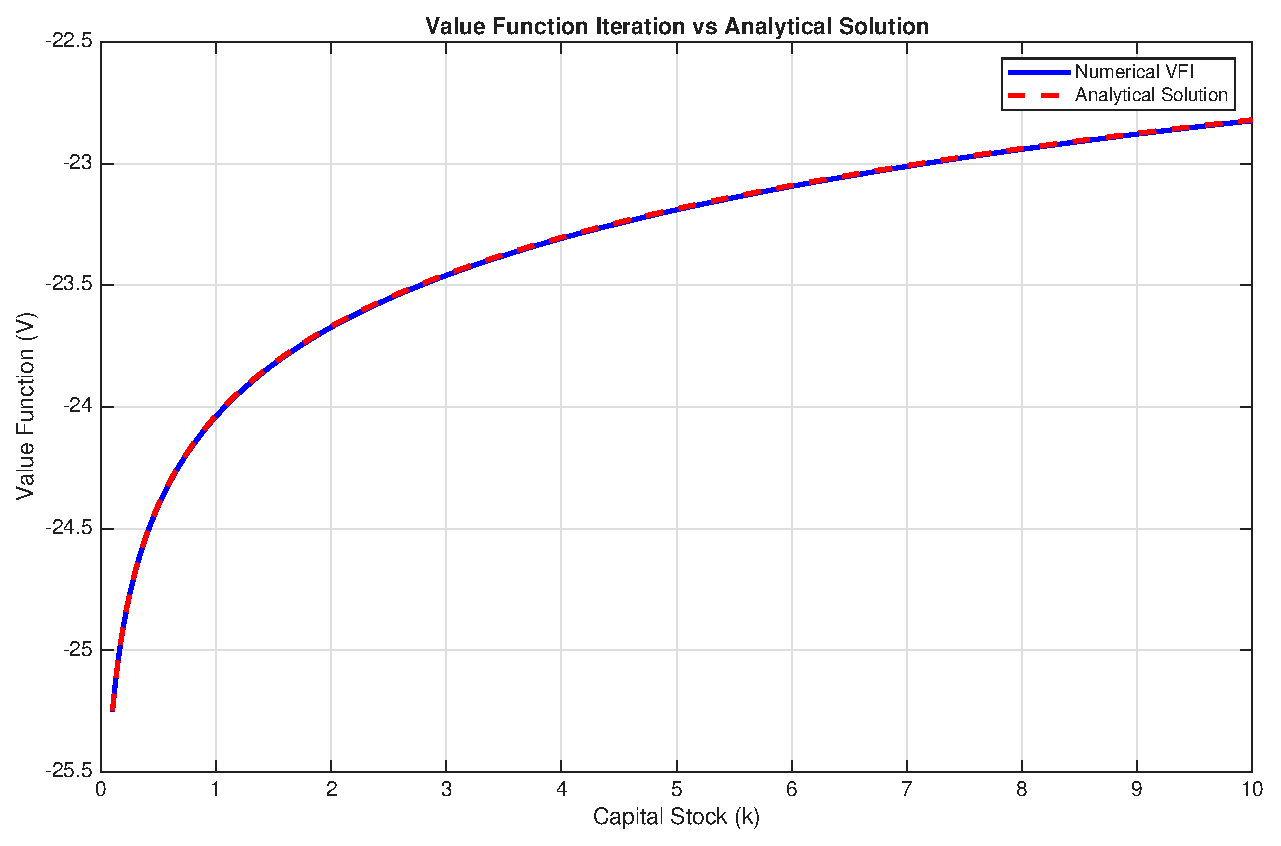
\includegraphics [width=4in]{PS2_Q1_02.eps}


\subsection*{Analytical policy function and other questions}

\begin{verbatim}
% calculaing max error between numerical and analytical policy functions
policy_analytical = analytical_policy_function(K_grid, Params); % calculate analytical policy function for comparison
disp('Analytical policy function at grid points:');
disp(policy_analytical(1:10));
max_policy_error = max(abs(policy_grid - policy_analytical)); % calculate maximum error between numerical and analytical policy functions
disp(['Maximum error between numerical and analytical policy functions: ', num2str(max_policy_error)]);

% does wealth grid bind?
if any(policy_grid == Params.point_a) || any(policy_grid == Params.point_b)
    disp('The wealth grid binds for some states.');
    finding_binding_indices = find(policy_grid == Params.point_a | policy_grid == Params.point_b); % find indices where policy function binds to the grid
    disp('The wealth grid binds at the following states:');
    disp(K_grid(finding_binding_indices)); % display the capital stock levels where the grid binds
else
    disp('The wealth grid does not bind for any states.');
end

% when does agent start deaccumalting wealth
% when k' < k?
deaccumulation_indices = find(policy_grid < K_grid); % find indices where policy function indicates deaccumulation of wealth
if ~isempty(deaccumulation_indices)
    disp('The agent starts deaccumulating wealth at');
    disp(K_grid(deaccumulation_indices(1))); % display the capital stock levels where deaccumulation starts
else
    disp('The agent does not deaccumulate wealth at any states.');
end
\end{verbatim}

        \color{lightgray} \begin{verbatim}Analytical policy function at grid points:
  Columns 1 through 7

    0.1501    0.1506    0.1522    0.1547    0.1582    0.1624    0.1673

  Columns 8 through 10

    0.1728    0.1787    0.1850

Maximum error between numerical and analytical policy functions: 0.027057
The wealth grid does not bind for any states.
The agent starts deaccumulating wealth at
    0.2010


ans =

    0.0200

\end{verbatim} \color{black}
    

\subsection*{Local Functions}

\begin{verbatim}
% creating funcion for the analytical value function
function V = analytical_value_function(k, Params)
    V = Params.a + Params.b * log(k); % analytical value function
end

% policy function
function k_prime = analytical_policy_function(k, Params)
    k_prime = Params.beta * Params.b *(Params.A * k.^Params.alpha +(1-Params.delta) * k) / (1 + Params.beta * Params.b); % analytical policy function
end
0.02
% making consumption function
function c = consumption(k, k_next, Params)
    c_possible = Params.A * k^Params.alpha - k_next + (1-Params.delta) * k; % possible consumption based on current capital, next period's capital, and production
    c = max(0, c_possible); % ensure consumption is non-negative
end

% utility function
function u = utility(c)
    u = -Inf(size(c));        % initialize all to -Inf
    u(c > 0) = log(c(c > 0)); % only compute log where feasible
end
\end{verbatim}

        \color{lightgray} \begin{verbatim}Analytical value function at grid points:
  Columns 1 through 7

  -25.2478  -25.2425  -25.2270  -25.2020  -25.1689  -25.1292  -25.0844

  Columns 8 through 10

  -25.0359  -24.9850  -24.9327

\end{verbatim} \color{black}
    


\end{document}

